\chapter{Ergebnisse}
\thispagestyle{fancy}

Im Folgenden sollen die Ergebnisse des KI-Modells nach den Gütekriterien evaluiert werden. Es wurden verschiedene Programme zur Analyse der Daten genutzt. Die grafische Aufbereitung der beim Training erfassten Fehlerwerte wurde mit der Software \textit{TensorBoard} \parencite{TensorBoard} durchgeführt. Statistiken entstanden in Python mittels der \textit{Pandas} \parencite{reback2020pandas} Programmbibliothek. 3D-Simulationsdaten verarbeiteten die Python-Module NumPy und OpenVDB. Für die visuelle Evaluation kam Houdini zum Einsatz. Es wurden insgesamt 23 Trainingsversuche durchgeführt und die Daten der letzten drei Trainingsversuche verglichen. Da diese ähnliche Graphen und Fehlerwerte erzeugten, bezieht sich die nachfolgende Evaluation nur auf den letzten Trainingsdurchlauf des KI-Modells.

\section{Evaluation der Gütekriterien}

\subsection{Artefaktfreiheit} Um die Ausgabe des Netzes auf visuelle Artefakte zu untersuchen, wurde eine neue, nicht im Training verwendete Simulation erzeugt. Es kam  dieselbe Vorgehensweise, wie für die Erzeugung der Trainingsdaten zum Einsatz. Die Simulation wurde erneut in 3D-Sub-Arrays und LowRes-3D-Arrays zerlegt, um eine niedrig aufgelöste Version zu erzeugen. Diese wurde anhand des trainierten KI-Modells hochskaliert und in ein OpenVDB konvertiert, um die Ursprungsgröße der Simulation zu erhalten. In Abbildung \ref{frame80}, einer Seitenansicht der Simulation, ist auf der rechten Seite die in Houdini erzeugte Simulation zu sehen und auf der linken Seite die durch die KI hochskalierte Version. Wie eindeutig zu erkennen, war das KI-Modell nicht in der Lage eine artefaktfreie Ausgabe zu erzeugen. Es generierte stattdessen eine Vielzahl an neuer Artefakte, wie etwa sich wiederholende Striche, welche rasterartig angeordnet sind. Ebenfalls waren einzelne, frei stehende Punkte sichtbar, die bei einer physikalisch korrekten Simulation nicht auftreten. Das Netz erzeugte eine gänzlich neue Form der Simulation, die nicht vergleichbar mit ihrem Ursprung ist.\\

\begin{figure}[ht]
    \centering
    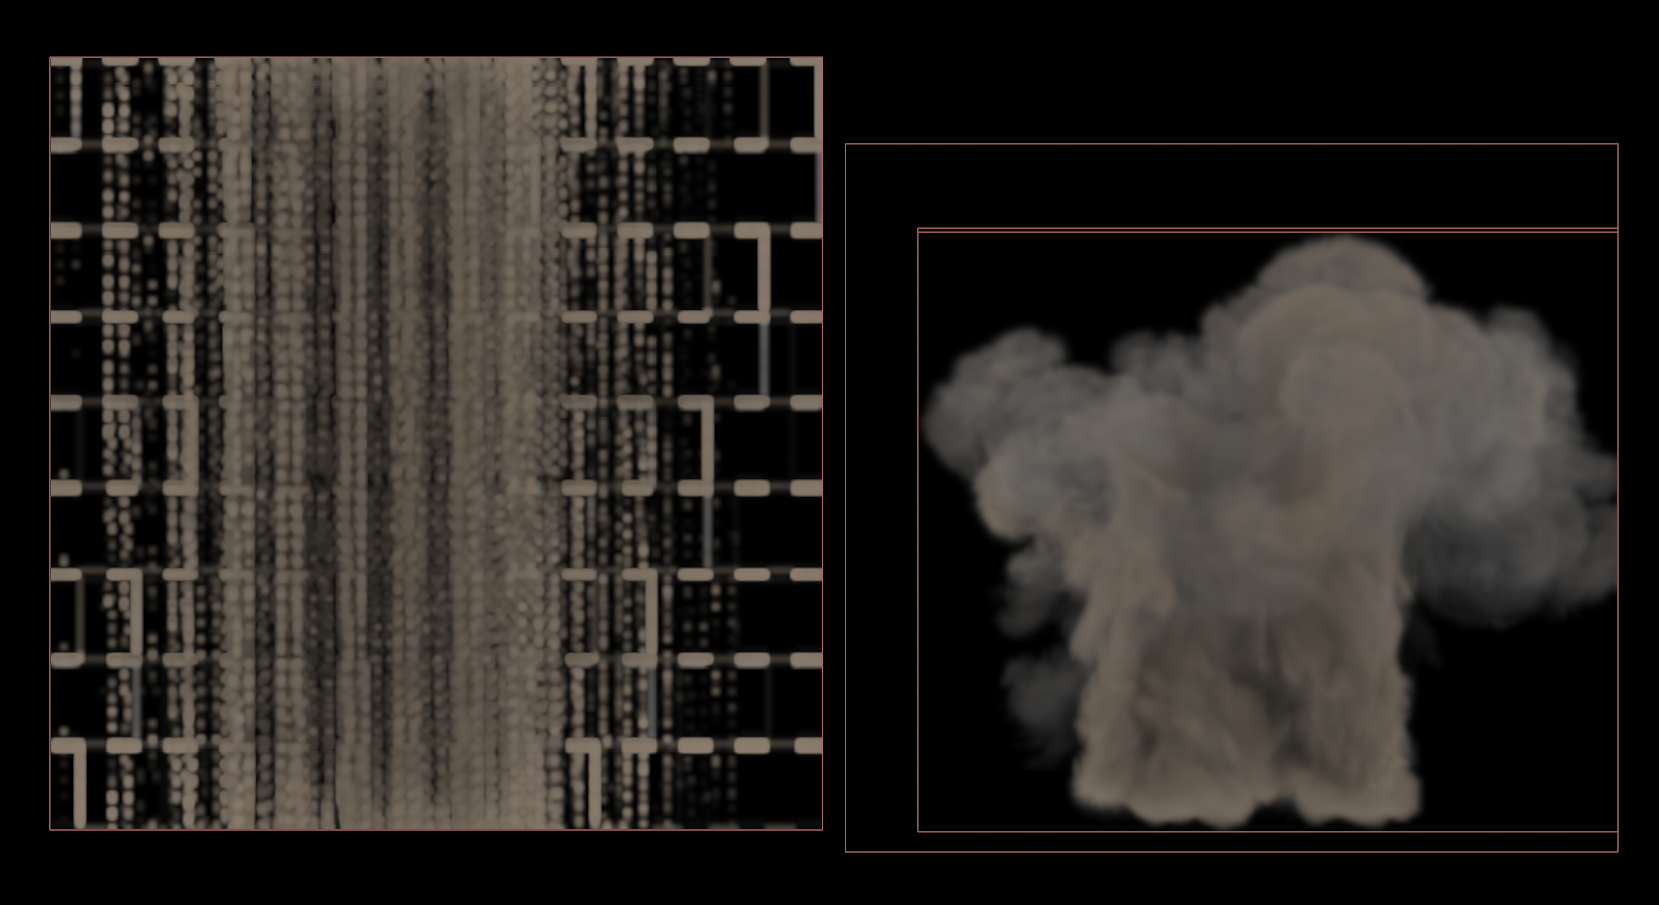
\includegraphics[width=14cm]{bilder/2Frame80.PNG}
    \caption{Detailansicht von Frame 80 der Simulationsvariante 2.}
    \source{Philipp Benner}
    \label{frame80}
\end{figure}

Das Kriterium der temporalen Kohärenz der Frames konnte ebenfalls nicht erfüllt werden, da einige Artefakte in jedem Frame an derselben Stelle sind. In Abbildung \ref{2scaled} ist der zeitliche Verlauf von zwei Simulationsvarianten zu sehen. Dargestellt sind jeweils Frame 1, Frame 40 und Frame 80. Sichtbar ist auch ein sich fortbewegender Streifen an dichten Voxeln, der über den Verlauf der Simulation von links nach rechts wanderte. Diese Form der Artefakte zeigte sich für alle getesteten Simulationsvarianten. \\

\begin{figure}[ht]
    \centering
    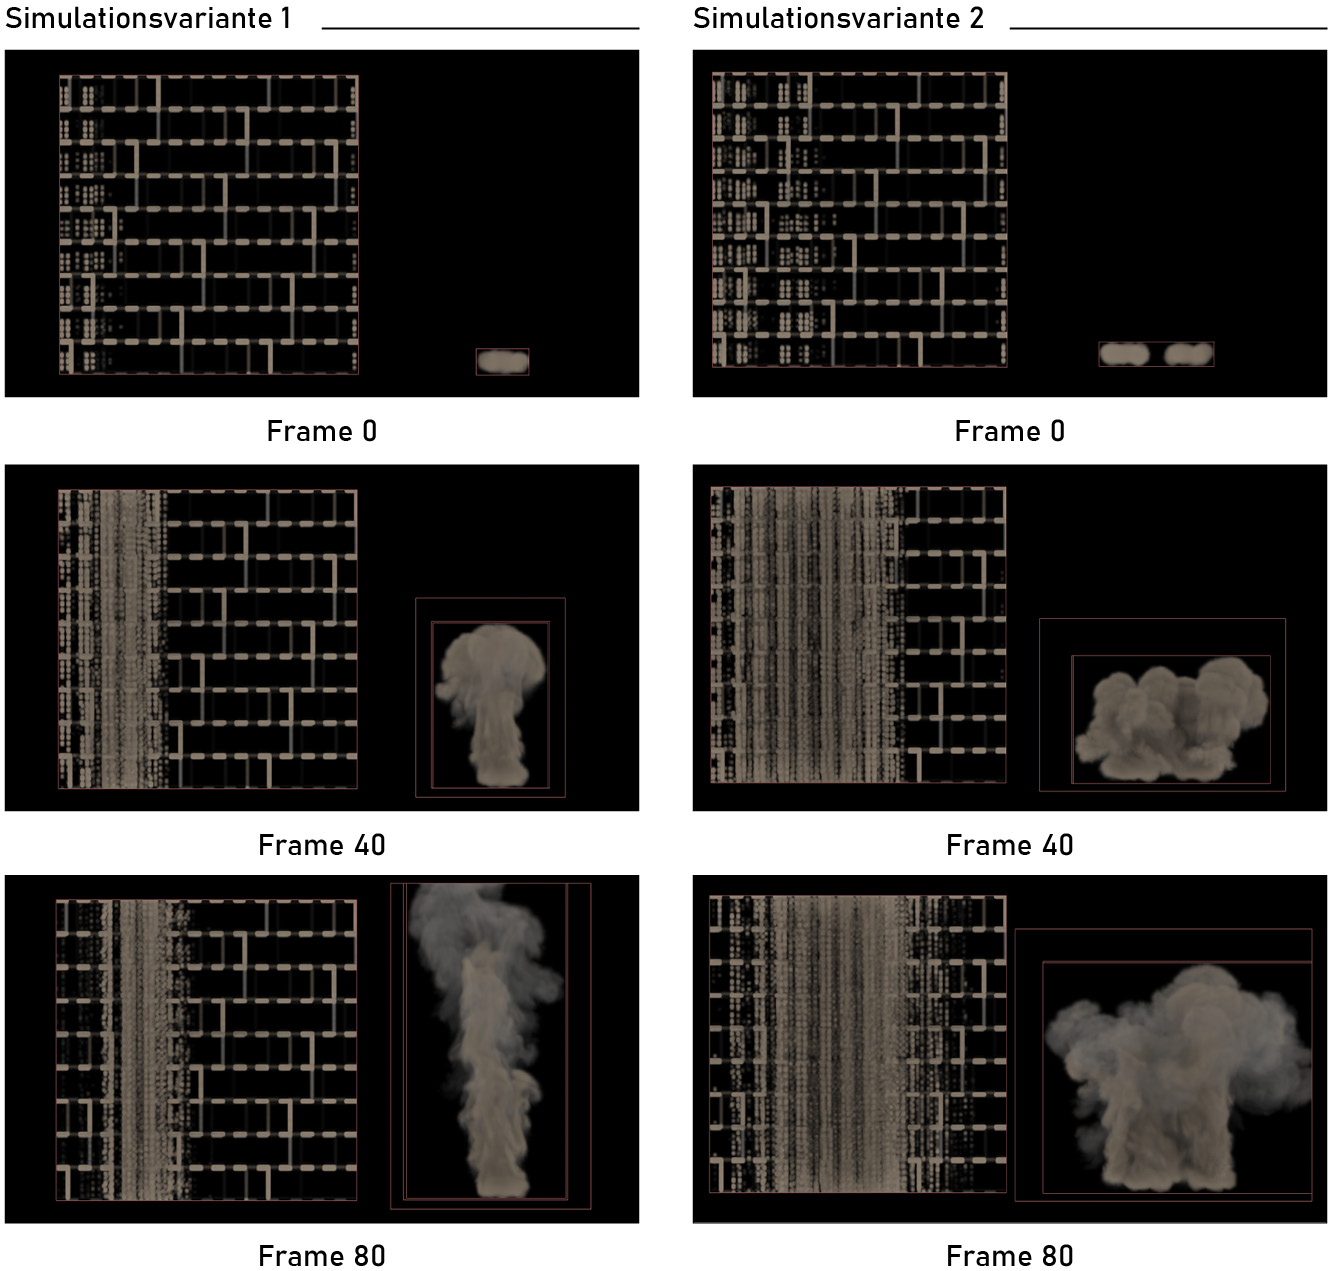
\includegraphics[width=13cm]{bilder/2_scaled_sims2.jpg}
    \caption{Vergleich einer Simulation mit einer hochskalierten Version derselben Simulation über die Zeit von 80 Frames.}
    \source{Philipp Benner}
    \label{2scaled}
\end{figure}
Hier zeigte sich das Problem des Mode Collapse, da das Netz eine ähnliche Ausgabe für jeden Frame erzeugte. Trotzdem ist sichtbar, dass das Netz trotz seiner Fehlerhaftigkeit in der Lage war, temporale Unterschiede zu erzeugen. Ein Grund für den Mode Collapse war möglicherweise die zufällige Selektion der 3D-Sub-Arrays. Da beim Training nicht alle Teile eines Frames verwendet wurden, war es möglich, dass viele Arrays durch den Discriminator und Generator geschleust wurden, die aus einer hohen Anzahl an Null-Werten bestanden. Das Netz war also nicht in der Lage eine physikalische Beziehung zwischen Density und Temperature Werten zu erlernen, da aussagekräftige Daten fehlten. Um dieses Problem zu lösen, müssten alle Teile eines Frames im Batch enthalten sein und nicht eine zufällige Auswahl an 3D-Sub-Arrays.\\

In Abbildung \ref{tensorboard} sind die Fehlerwerte oder Loss des Discriminators und Generators zu sehen. Sie waren das Ergebnis des Optimizers nach dem Training. Zur Messung der Fehlerwerte des Generators wurden echte sowie künstliche Daten durch den Generator geschleust und dessen Output anschließend vom Discriminator klassifiziert. Für die linken Graphen der Abbildung \ref{tensorboard} stellt die \textit{y}-Achse der Fehlerwert und die \textit{x}-Achse die Anzahl an trainierten Batches dar. Zu sehen ist ebenfalls, dass nur circa 1400 Batches trainiert wurden. Der Grund hierfür ist, dass sich früh abzeichnete, dass das Netz nicht optimal trainiert und deshalb das Training abgebrochen wurde. Der Generator erzeugte beispielsweise einen Fehlerwert von unter 0,1 innerhalb der ersten 200 Batches. Das drückt aus, dass sich der Discriminator sehr sicher ist, künstliche Daten klassifiziert zu haben. In diesem frühen Stadium des Trainings sind extreme Werte zur Klassifizierung ein Zeichen für ein schlecht trainierendes Netz. Die rechte Spalte der Abbildung \ref{tensorboard} zeigt auf ihrer y-Achse die Werte am Ausgang des Discriminators, basierend auf seinen Input-Daten. Dieser Wert unterscheidet sich dahingehend vom Fehlerwert, als dass er nicht das Ergebnis des Optimizers war, sondern der reine Output am letzten Layer des Modells. Die \textit{x}-Achse stellt die Anzahl der trainierten Batches dar. \\

\begin{figure}[ht]
    \centering
    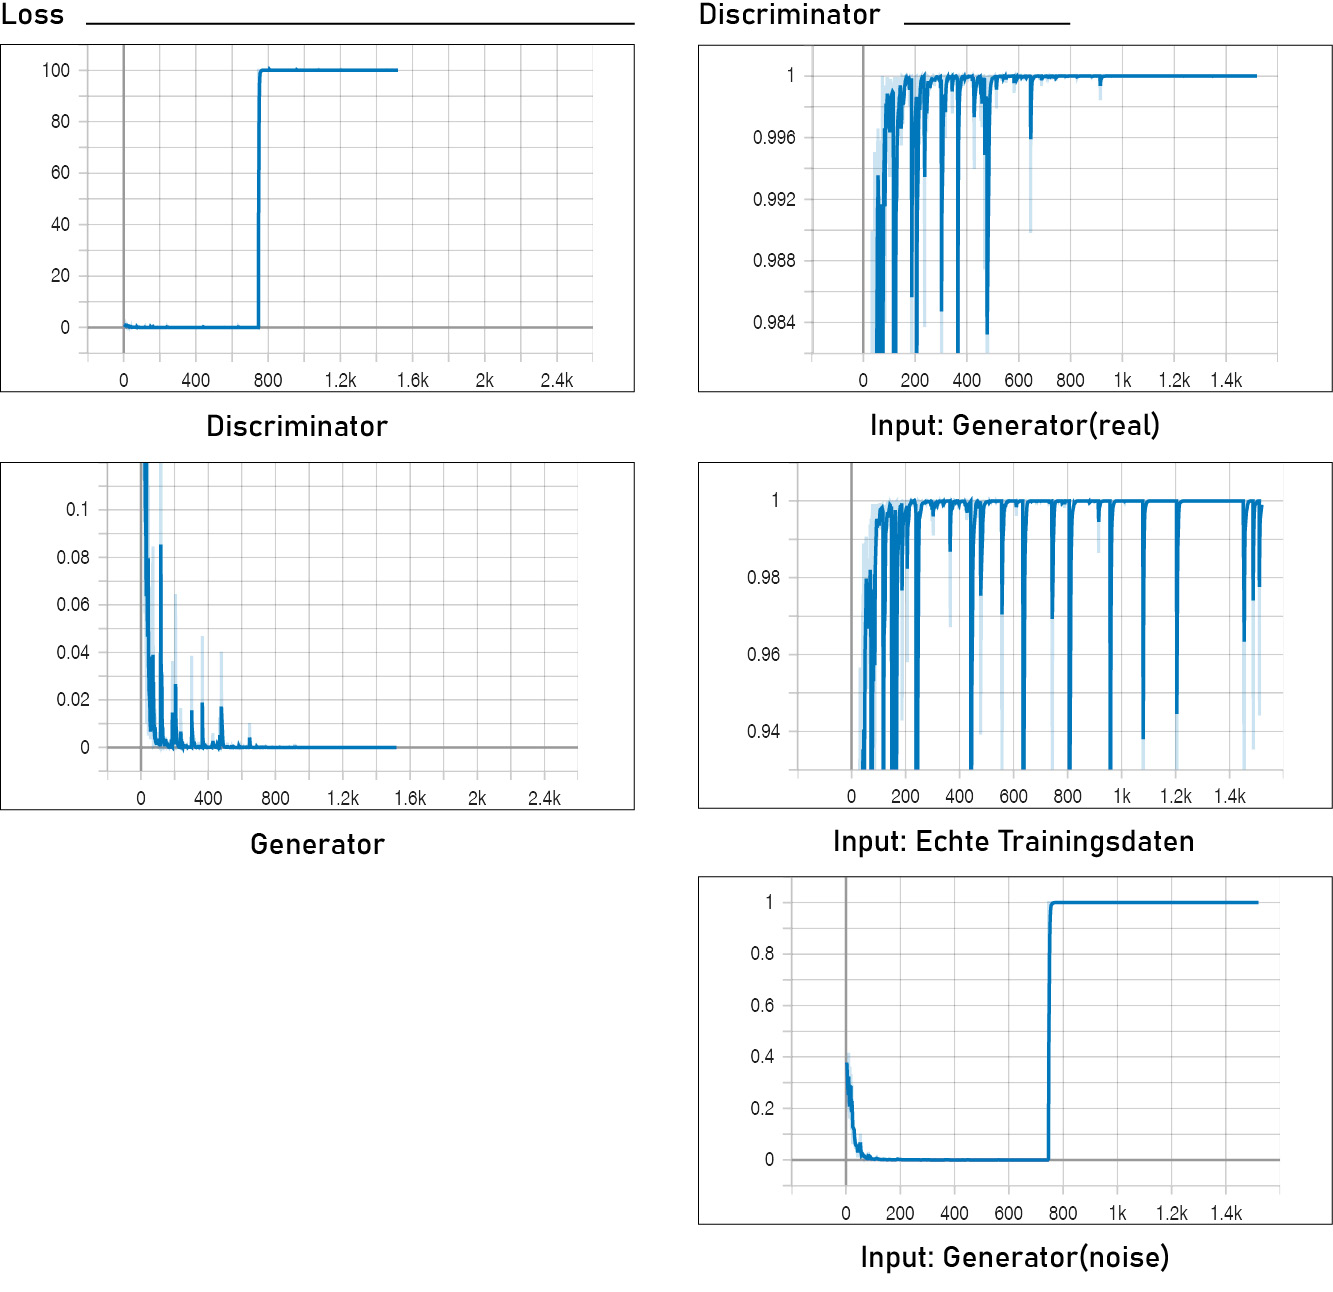
\includegraphics[width=13cm]{bilder/tensorboard2.jpg}
    \caption{Fehlerwerte des Generators und Discriminators.}
    \source{Philipp Benner}
    \label{tensorboard}
\end{figure}

Der obere, rechte Graph zeigt den Wert des Discriminators, wenn ihm ein Generator-Output gezeigt wurde, der mit echten Daten im Generator erzeugt wurde. Hier erreichen die Werte nach wenigen Batches einen Wert nahe 1, was bedeuten würde, dass der Generator optimal trainieren konnte, da der Discriminator sich sicher ist, echte Daten zu erkennen. Nach kurzer Trainingsdauer ist dies ebenfalls kein optimales Ergebnis.\\

Im mittleren Graphen zeigt sich die Entwicklung des Discriminators, als er direkt mit echten Daten trainiert wurde und nicht über den Output des Generators. Hier zeigte sich ebenfalls das Problem der extremen Werte in einem frühen Stadium des Trainings. Über den Verlauf des Trainings werden hier Einbrüche des Wertes im Graphen sichtbar.Diese bedeuten, dass sich der Discriminator bei einigen Batches nicht sicher war, ob die Daten echt sind. \\

Der untere Graph gibt den Wert des Discriminators an, als an diesen falsche Daten aus dem Generator angelegt wurden. Diese Daten wurden mit einem Noise erzeugt, dass der Generator hochskalierte. Erneut ist zu sehen, dass sich der Discriminator sehr früh sicher war, diese Daten als falsch klassifizieren zu können. Nach circa 750 Batches steigt der Wert jedoch auf nahezu 1,0. Dieser Sprung zeigt sich auch im Graphen für den Loss des Discriminators. Ein Vergleich mit den anderen Graphen zeigte, dass circa nach dem 750. Batch eine Veränderung im Generator auftrat. Der mittlere Graph der rechten Spalte zeigt keine sprunghafte Veränderung seiner Werte nach diesem Zeitpunkt, da dieser nicht auf dem Output des Generators basierte. Möglicherweise stellt dies den Zeitpunkt des Mode Collapse dar und der Generator lernte einen Output zu erzeugen, der stets mit annähernd 1,0 klassifiziert werden konnte. Ein Punkt, der diese Behauptung stützt, sind die sichtbaren, zufälligen Artefakte, die in Abbildung \ref{frame80} zu sehen sind.\\

Es lässt sich somit festhalten, dass das Kriterium der Artefaktfreiheit nicht erfüllt werden konnte.

\subsection{Formgleichheit} Das Kriterium der Formgleichheit ist ebenfalls nicht erfüllt, da aus den im Abschnitt zur Artefaktfreiheit genannten Gründen kein visuell korrekter Output erzeugt werden konnte. Die Form der Output-Simulation ist, wie in Abbildung \ref{frame80}, nicht mit ihrer Ursprungsform vergleichbar.\\

\subsection{Schnelligkeit}
Zur Evaluation der Schnelligkeit wurden, basierend auf den vorherigen Prozessen zu Erstellung von Trainingsdaten, drei neue Varianten an Simulationen in Houdini erzeugt. Jede Simulation bestand aus 80 Frames, die zu einem NumPy-Array der Auflösung 208 $\cdot$ 208 $\cdot$ 208 $\cdot$ Voxel konvertiert und in eine Low Resolution Version gewandelt wurden, anschließend mit dem KI-Modell hochskaliert und in das OpenVDB Format konvertiert, um die ursprüngliche Simulation wiederherzustellen.\\

Die Zeit, um eine Low Resolution Version aus einer Simulation zu erzeugen, sei zu vernachlässigen, da Tests zeigten, dass die Interpolation zu einer geringeren Auflösung hin circa eine Millisekunde betrug.\\

Es wurde anhand eines Python-Skripts analysiert, zu welchem Zeitpunkt ein Frame der originalen Simulation und ein Frame der KI-Skalierung erstellt wurde. Anhand von diesen Werten ließ sich ableiten, wie lange es dauerte, eine komplette Simulation in Houdini zu simulieren und ebenso die Zeit messen, die das KI-Modell zum Skalieren aller Frames benötigte. Ein Python-Skript berechnete ebenfalls die benötigte Zeit über alle Frames, da die anfänglichen Frames in Houdini weniger Zeit für die Simulation benötigen, als die Frames am Ende. Diese ersten Frames bestanden aus einer geringeren Anzahl an aktiven Voxeln in der Simulation. Somit mussten weniger Berechnungen am zu Beginn durchgeführt werden. In den Tabellen \ref{tab:speed} sind die gesamte Simulations- und Upsampling-Zeit und die durchschnittliche Dauer pro Frame von Houdini und des KI-Modells zu sehen. In der letzten Zeile wurde der Gesamtdurchschnitt der drei Werte gebildet. \\

\begin{table}[h]
    \centering
    \caption{Vergleich der Durchschnittsdauer eines simulierten und eines hochskalierten Frames.}
\begin{tabular}{|r|c|c|}
    
\hline
   & \multicolumn{2}{c|}{Houdini} \\
   \hline
           &  Simulationsdauer [s]       & 	$\varnothing$ Dauer pro Frame [s]\\
            \hline
Variante 1 & 29 Sek.          & 0,36 Sek.                       \\
Variante 2 & 19 Sek.          & 0,24 Sek.                      \\
Variante 3 & 21 Sek.           & 0,26 Sek.                       \\
\hline
\hline
 $\varnothing$   &     23 Sek.      &  0,27 Sek.           \\
 \hline
\end{tabular}
\vspace{0.7cm}\\
\begin{tabular}{|r|c|c|}
    
\hline
   &\multicolumn{2}{c|}{Upsampling} \\
   \hline
            & Dauer [s]      & 	$\varnothing$ Dauer pro Frame [s]        \\
            \hline
Variante 1     &  1 Min. 18 Sek.         & 0,97 Sek.             \\
Variante 2         &   1 Min. 12 Sek.        &  0,90 Sek.            \\
Variante 3          &  1 Min. 13 Sek.         &  0,91 Sek.           \\
\hline
\hline
 $\varnothing$   &    1 Min. 14 Sek.       &    0,93 Sek.    \\
 \hline
\end{tabular}

    \label{tab:speed}
\end{table}

Der Tabelle \ref{tab:speed} ist zu entnehmen, dass es etwa um den Faktor drei schneller war, einen Frame in Houdini zu simulieren, anstatt diesen mit dem KI-Modell zu skalieren. Dieser Zeitvorteil entsteht, da Houdini nicht jeden Voxel innerhalb des 3D-Arrays berechnete, sondern nur aktive Voxel mit Density und Temperature Werten \parencite{sidefxsparse}. Das KI-Modell hingegen hatte die Form eins 3D-NumPy-Arrays, dessen Werte alle in Input-Neuronen gewandelt werden mussten. Somit führte das KI-Modell immer eine Berechnung für die komplette Größe des Arrays durch und benötigte deshalb mehr Zeit.\\

Trotzdem ist es möglich, die Simulation schneller zu skalieren, als sie mit Houdini zu simulieren. Das KI-Modell hat den Vorteil, dass es parallel alle Frames zur selben Zeit skalieren kann. Dazu müssten mehrere Programminstanzen des Python-Skripts erstellt werden und jede Instanz würde einen Frame skalieren. Da das KI-Modell eine leistungsfähige, NVIDIA Grafikkarte pro Instanz benötigt, ist dieses Vorgehen beispielsweise nur auf einer Rechenfarm mit mehreren Grafikkarten möglich. Basierend auf den Werten aus Tabelle \ref{tab:speed} ließe sich die Simulationsvariante 1 ab vier Programminstanzen schneller hochskalieren, als Houdini durchschnittlich an Simulationszeit benötigt. Wie im Abschnitt zu Simulationen erläutert wurde, simuliert Houdini alle Frames nacheinander, da die Berechnungen eines Frames auf dem vorhergehenden Frame basieren. Diese Methode lässt sich nicht durch mehrere Houdini-Instanzen aufteilen.\\

Das Kriterium der Schnelligkeit ist somit erfüllt, sofern das KI-Modell zur parallelen Erzeugung von Frames genutzt wird.

\subsection{Datensparsamkeit}
Ob das Netz in die Fähigkeit hat, ein korrektes Upsampling von Simulationen mit dem Density und Temperature Field einer Simulation durchzuführen, ließ sich nicht evaluieren, da keine visuell korrekte Ausgabe erzeugt werden konnte. Somit ist das Kriterium der Datensparsamkeit nicht erfüllt.

\section{Vergleich mit tempoGAN}
Die Autoren der tempoGAN Implementierung zeigten jedoch, dass es durchaus möglich ist ein visuell artefaktfreies Upsampling über neuronale Netze zu erreichen \parencite[S. 95:10]{xie2018tempoGAN}. Die dort erzeugten Ergebnisse des Upsampling zeigten eine hohe zeitliche Kohärenz und einen sichtbaren Detailgrad in den Simulationen der erhöhten Auflösung.\\

Bei einer Evaluation der temoGAN Implementierung mit den Gütekriterien dieser Forschungsarbeit, ließe sich ein positives Ergebnis für die Artefaktfreiheit und Formgleichheit festhalten. Das Upsampling im tempoGAN Modell ist ebenso in einer hohen Geschwindigkeit möglich. Laut den Autoren dauerte die Simulation eines Frames in Mantaflow circa 31,5 Minuten, wohingegen das Upsampling des Low Resolution Frames durch das Netz nur 3,9 Minuten dauerte \parencite[S. 95:13]{xie2018tempoGAN}. \\

Ohne weitere Experimente lässt sich dieses Kriterium im VFX-Bereich nicht eindeutig testen, jedoch bietet es einen weiteren Forschungsanreiz.\\

Das Kriterium der Datensparsamkeit konnte durch die tempoGAN Implementierung nicht erfüllt werden, da dort das Velocity anstatt des Temperature Fields eingesetzt wurde. Wie in Tabelle \ref{tab:veltemp} gezeigt, benötigte die Kombination aus Density und Velocity Field mehr Speicherplatz als das Density und Temperature Field.

\section{Fazit und Lösungsansatz}
Die Evaluation der Gütekriterien zeigte, dass es nicht möglich war ein optimales KI-Modell für das Upsampling von Rauchsimulationen, basierend auf der Forschungsfrage, zu trainieren. Die Gründe hierfür sind vielseitig und ließen sich nicht an einer einzelnen Fehlerquelle festmachen. Jedoch lässt sich eine Artefaktfreiheit und die temporale Kohärenz mit weiterer Forschung erreichen, da eine Optimierung des KI-Modells ist durchaus möglich ist. \\

Optimierungsansätze liegen beispielsweise in der Batch Size und Hardwareleistung. Auf einer Grafikkarte, die über mehr Speicherplatz verfügt, ließen sich alle Frames durch das Netz schleusen, anstatt nur eine Selektion an 3D-Sub-Arrays. Ebenfalls ließe sich das KI-Modell auf einer Farm trainieren, auf der möglicherweise mehr als ein Frame Teil eines Batches sein könnte oder es ließen sich mehr Trainingsepochen in kürzerer Zeit realisieren. Eine weitere Möglichkeit zur Optimierung liegt im Aufbau des Discriminators und des Generators. Wie im Abschnitt der Implementierung des Generators beschrieben, wurden für diesen mehr Convolutional und Residual Layer verwendet als beim Discriminator. Dadurch entstand das Problem, dass die beiden Kontrahenten nicht gleich stark und der Generator überlegen war. Er erhielt vom Discriminator kein ausreichendes Feedback, um sich in einer Weise zu verbessern, die visuell artefaktfreie Ergebnisse erzeugt.\\

Die Ergebnisse der tempoGAN Implementierung zeigen aber deutlich, dass ein Upsampling mittels neuronaler Netze möglich ist. Da die Autoren den Quellcode offengelegt und den Aufbau des KI-Models sehr genau beschrieben haben, kann dieses KI-Modell mit weiterer Entwicklung in eine Software des VFX-Bereichs integriert werden. Ein Mittel dafür stellt das Python-Modul des OpenVDB Herstellers dar, da dieses die Datenkonvertierung zwischen OpenVDB und einem NumPy-Array stark vereinfacht. Somit ließen sich diverse Python-Skripte in Houdini implementieren, die eine solche Aufgabe übernehmen könnten.